
% ################################# Paragraph #################################
% Short introduction into the cataylsis section
In the following section we will demonstrate the merit of our bulk crystal searching method by investigating the 4 most stable structures for the OER, an important electrochemical reaction with application in energy storage technologies.


% | - Bulk Pourbaix
\subsubsection{Bulk Pourbaix}

% ################################# Paragraph #################################
% COMBAK
% QUESTION Use E or U for potential variable
The electrochemical stability phase diagram (E vs. pH) was constructed by considering the equilibrium conditions of the following species: Ir, \rIrOtwo, \aIrOthree, \rIrOthree, \bIrOthree, and an aqueous dissolved \ce{IrO[4-]} species (See TEMP|SI for additional details).
The resulting diagram is shown in Fig. \ref{fig:bulk_pourbaix}.
Importantly, under acidic conditions (pH < 7) and in the bias region of interest for the OER (~1.23 V vs. RHE) \aIrOthree shows a large window of stability.
This indicates that the \aIrOthree phase may be stabilized under the highly oxidizing conditions of the OER.
The stability regions for \rIrOthree and \bIrOthree in the absence of any other \ce{IrO_3} polymorphs are also indicated by the unfilled solid lines and demonstrate a sizable stability window as well.
This result implies that these metastable phases may also play a role for the OER.
% Also explain the Ir and IrO[4-] ion

% | - Figure | Bulk Pourbaix Diagram
\begin{figure}
\centering
\makebox[\textwidth][c]{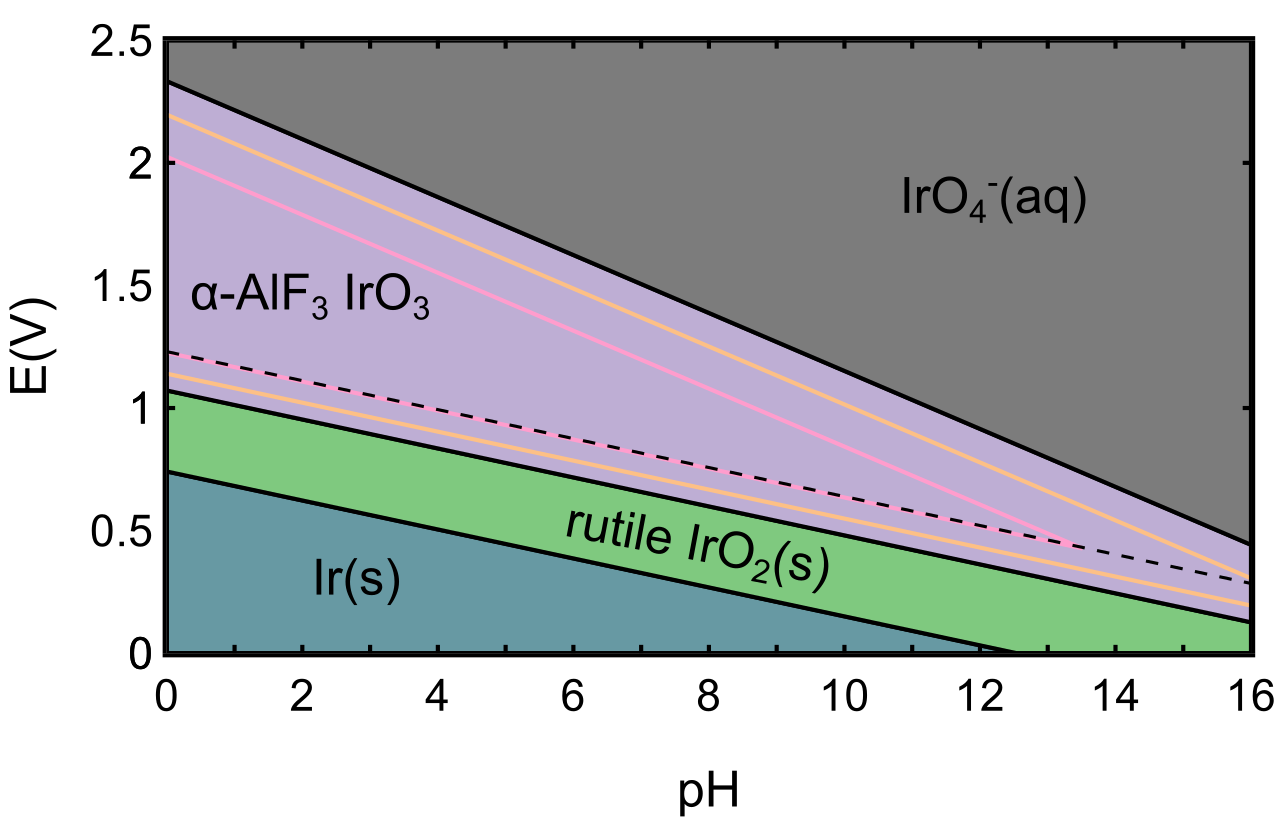
\includegraphics
{02_figures/oer_activity_stability/00_master__bulk-pourbaix__v1__400dpi__0__outplot.png}
% {02_figures/oer_activity_stability/bulk_pourbaix_0.pdf}
}
\caption{\label{fig:bulk_pourbaix}
Electrochemical bulk phase stability diagram (Pourbaix) of the Ir-O-H chemical space considering rutile-\ce{IrO_2},
}
\end{figure}
% __|

% __|

% | - OER Activities and Surfaces
\subsubsection{b. OER Activities and Surfaces}

% ################################# Paragraph #################################
% Surface Energy Pourbaix Analysis
The OER activity (expressed in terms of the limiting potential) for various surfaces cut from rutile-\ce{IrO_2}, and the three polymorphs of \ce{IrO_3} considered are shown in Fig. \ref{fig:oer_volcano}.
% TODO #REF | Reference for VESTA x-ray diff. pattern method
The specific facets were chosen from the highest intensity x-ray diffraction peaks from powder-diffraction spectra simulated in VESTA,
as well as using physical intuition as to which facets would be most physical.


% | - Figure | OER Volcano/Surface Pourbaix
\begin{figure}
\centering
\makebox[\textwidth][c]{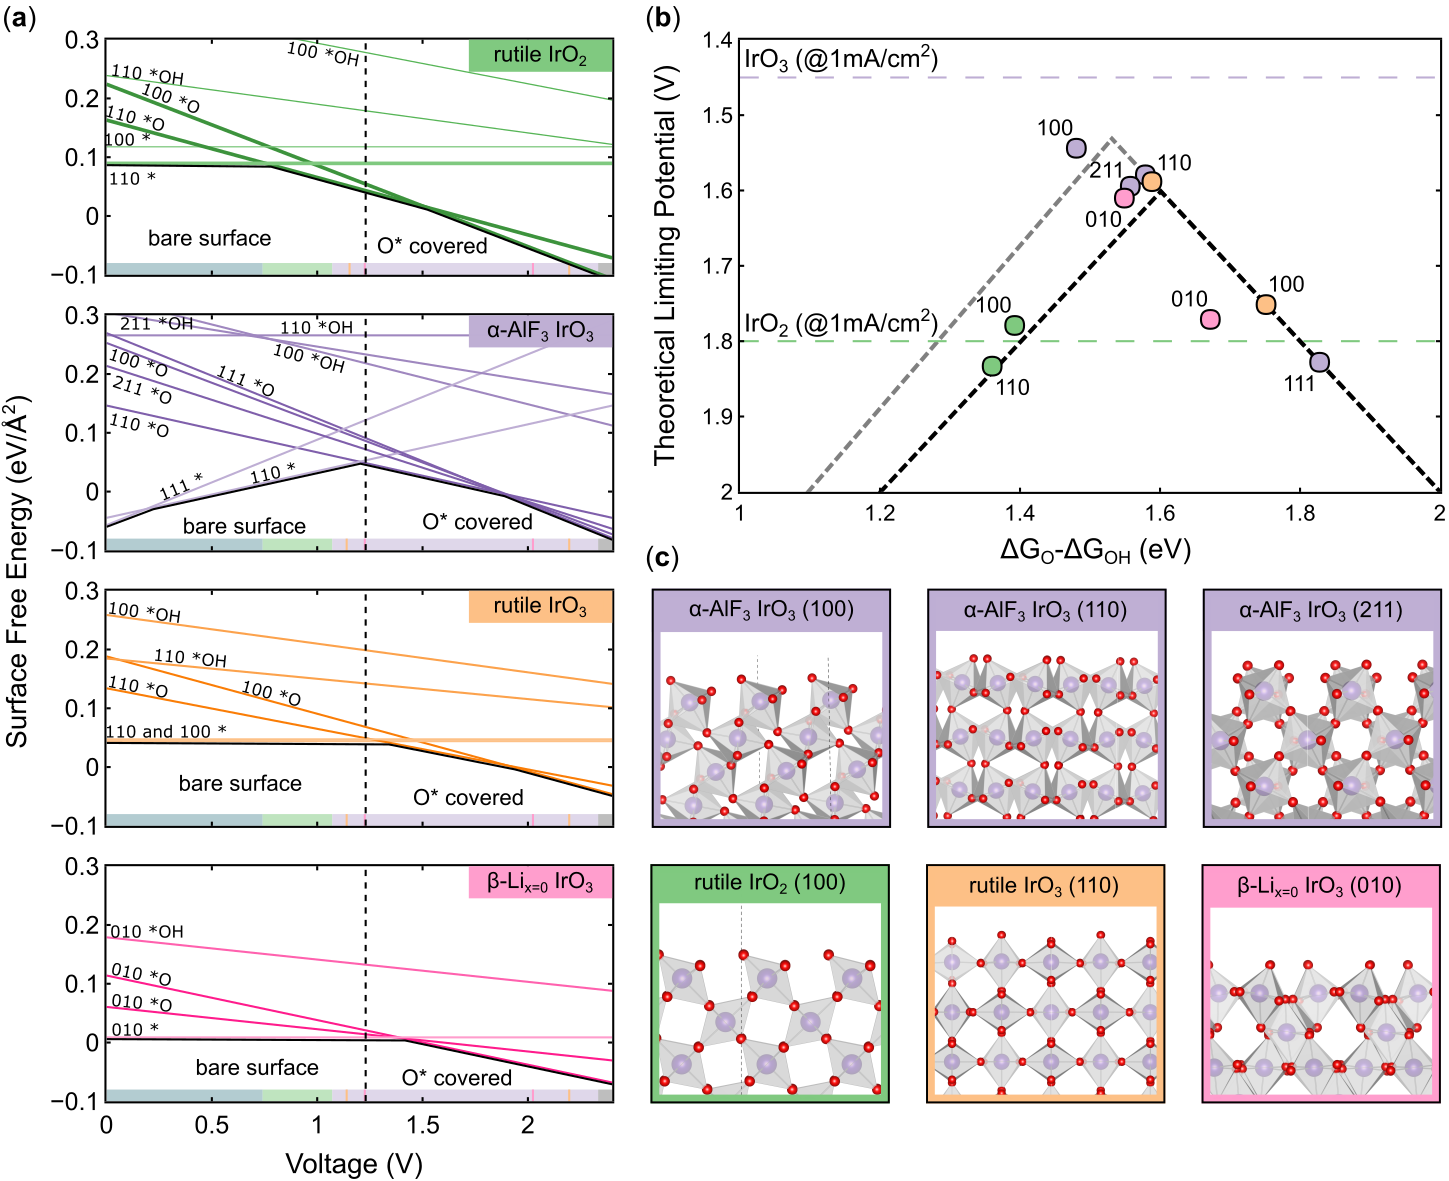
\includegraphics
{02_figures/oer_activity_stability/00_master__oer-volc_surf-pourb_struct__main_v3__200dpi__outplot.png}
% {02_figures/oer_activity_stability/00_master_plot__oer-volc_surf-pourb_struct__main_v3__outplot.pdf}
}
\caption{\label{fig:oer_volcano}
Summary of OER results for the four bulk structures of \IrOx considered: rutile-\ce{IrO_2} (green), $\alpha$-\ce{IrO_3} (purple), rutile-\ce{IrO_3} (orange), and $\beta$-\ce{IrO_3} (pink).
% -----------------------------------------------------------------------------
(a) Surface energy Pourbaix diagrams for each structure, with the surface energy of various facets and coverages shown as a function of applied potential.
The bulk Pourbaix diagram's bounds of stability at pH 0 are superimposed at the bottom of each subplot.
% -----------------------------------------------------------------------------
(b) OER activity volcano for \IrOx systems considered utilizing the \DGOmOH thermodynamic descriptor.
The purple dotted line corresponds to the experimental limiting potential at 10 mA cm\textsuperscript{2} for \ce{IrO_3}, % #TODO #REF Insert Seitz Science reference
while the green band corresponds to the range of experimentally observed overpotentials for pristine \ce{IrO_2} catalysts.  % TODO Insert green band into figure
% -----------------------------------------------------------------------------
(c) Select surface facets for the four \IrOx crystal systems considered.
% -----------------------------------------------------------------------------
% | - __old__
% Circles designate oxygen covered surfaces while triangles designate hydroxyl (*OH) terminated surfaces (relevant surface terminations were found via surface Pourbaix analyses).
% Surface energies at standard conditions (pH and V = 0) are reflected in the border color for each data point, where black indicates a low energy surface termination and white indicates more unstable surfaces.  % Currently not implemented as this
% The color range goes from x to y.
% __|
}
\end{figure}
% __|

% ################################# Paragraph #################################
To determine the most likely experimentally abundant surface facets and surface coverages, a surface energy Pourbaix diagram was constructed (TEMP).  % COMBAK Insert correct reference
See (SI for surface energy/Pourbaix part) for the method used to calculate surface energies.
% COMBAK
% __|

% | - OER Scaling Relations
\subsubsection{c. OER Intermediate Scaling}

% ################################# Paragraph #################################
Figure TEMP shows the scaling relations between the adsorption free energies of the OER intermediate species for the \IrOx systems studied herein.
It can be seen clearly that the data points corresponding to the three \ce{IrO_3} polymorphs are roughly 1 eV weaker binding than the rutile-\ce{IrO_2} points.
This generally weaker binding of the \ce{IrO_3} stoichiometry is responsible for the observed improvement in theoretical activity.
The \DGOOH vs.\DGOH relationship is very close to the traditional ``universal scaling relations'', demonstrating that our materials do not break the infamous \DGOOH vs. \DGOH scaling.

% | - Figure | OER Scaling Relations
\begin{figure}
\centering
\makebox[\textwidth][c]{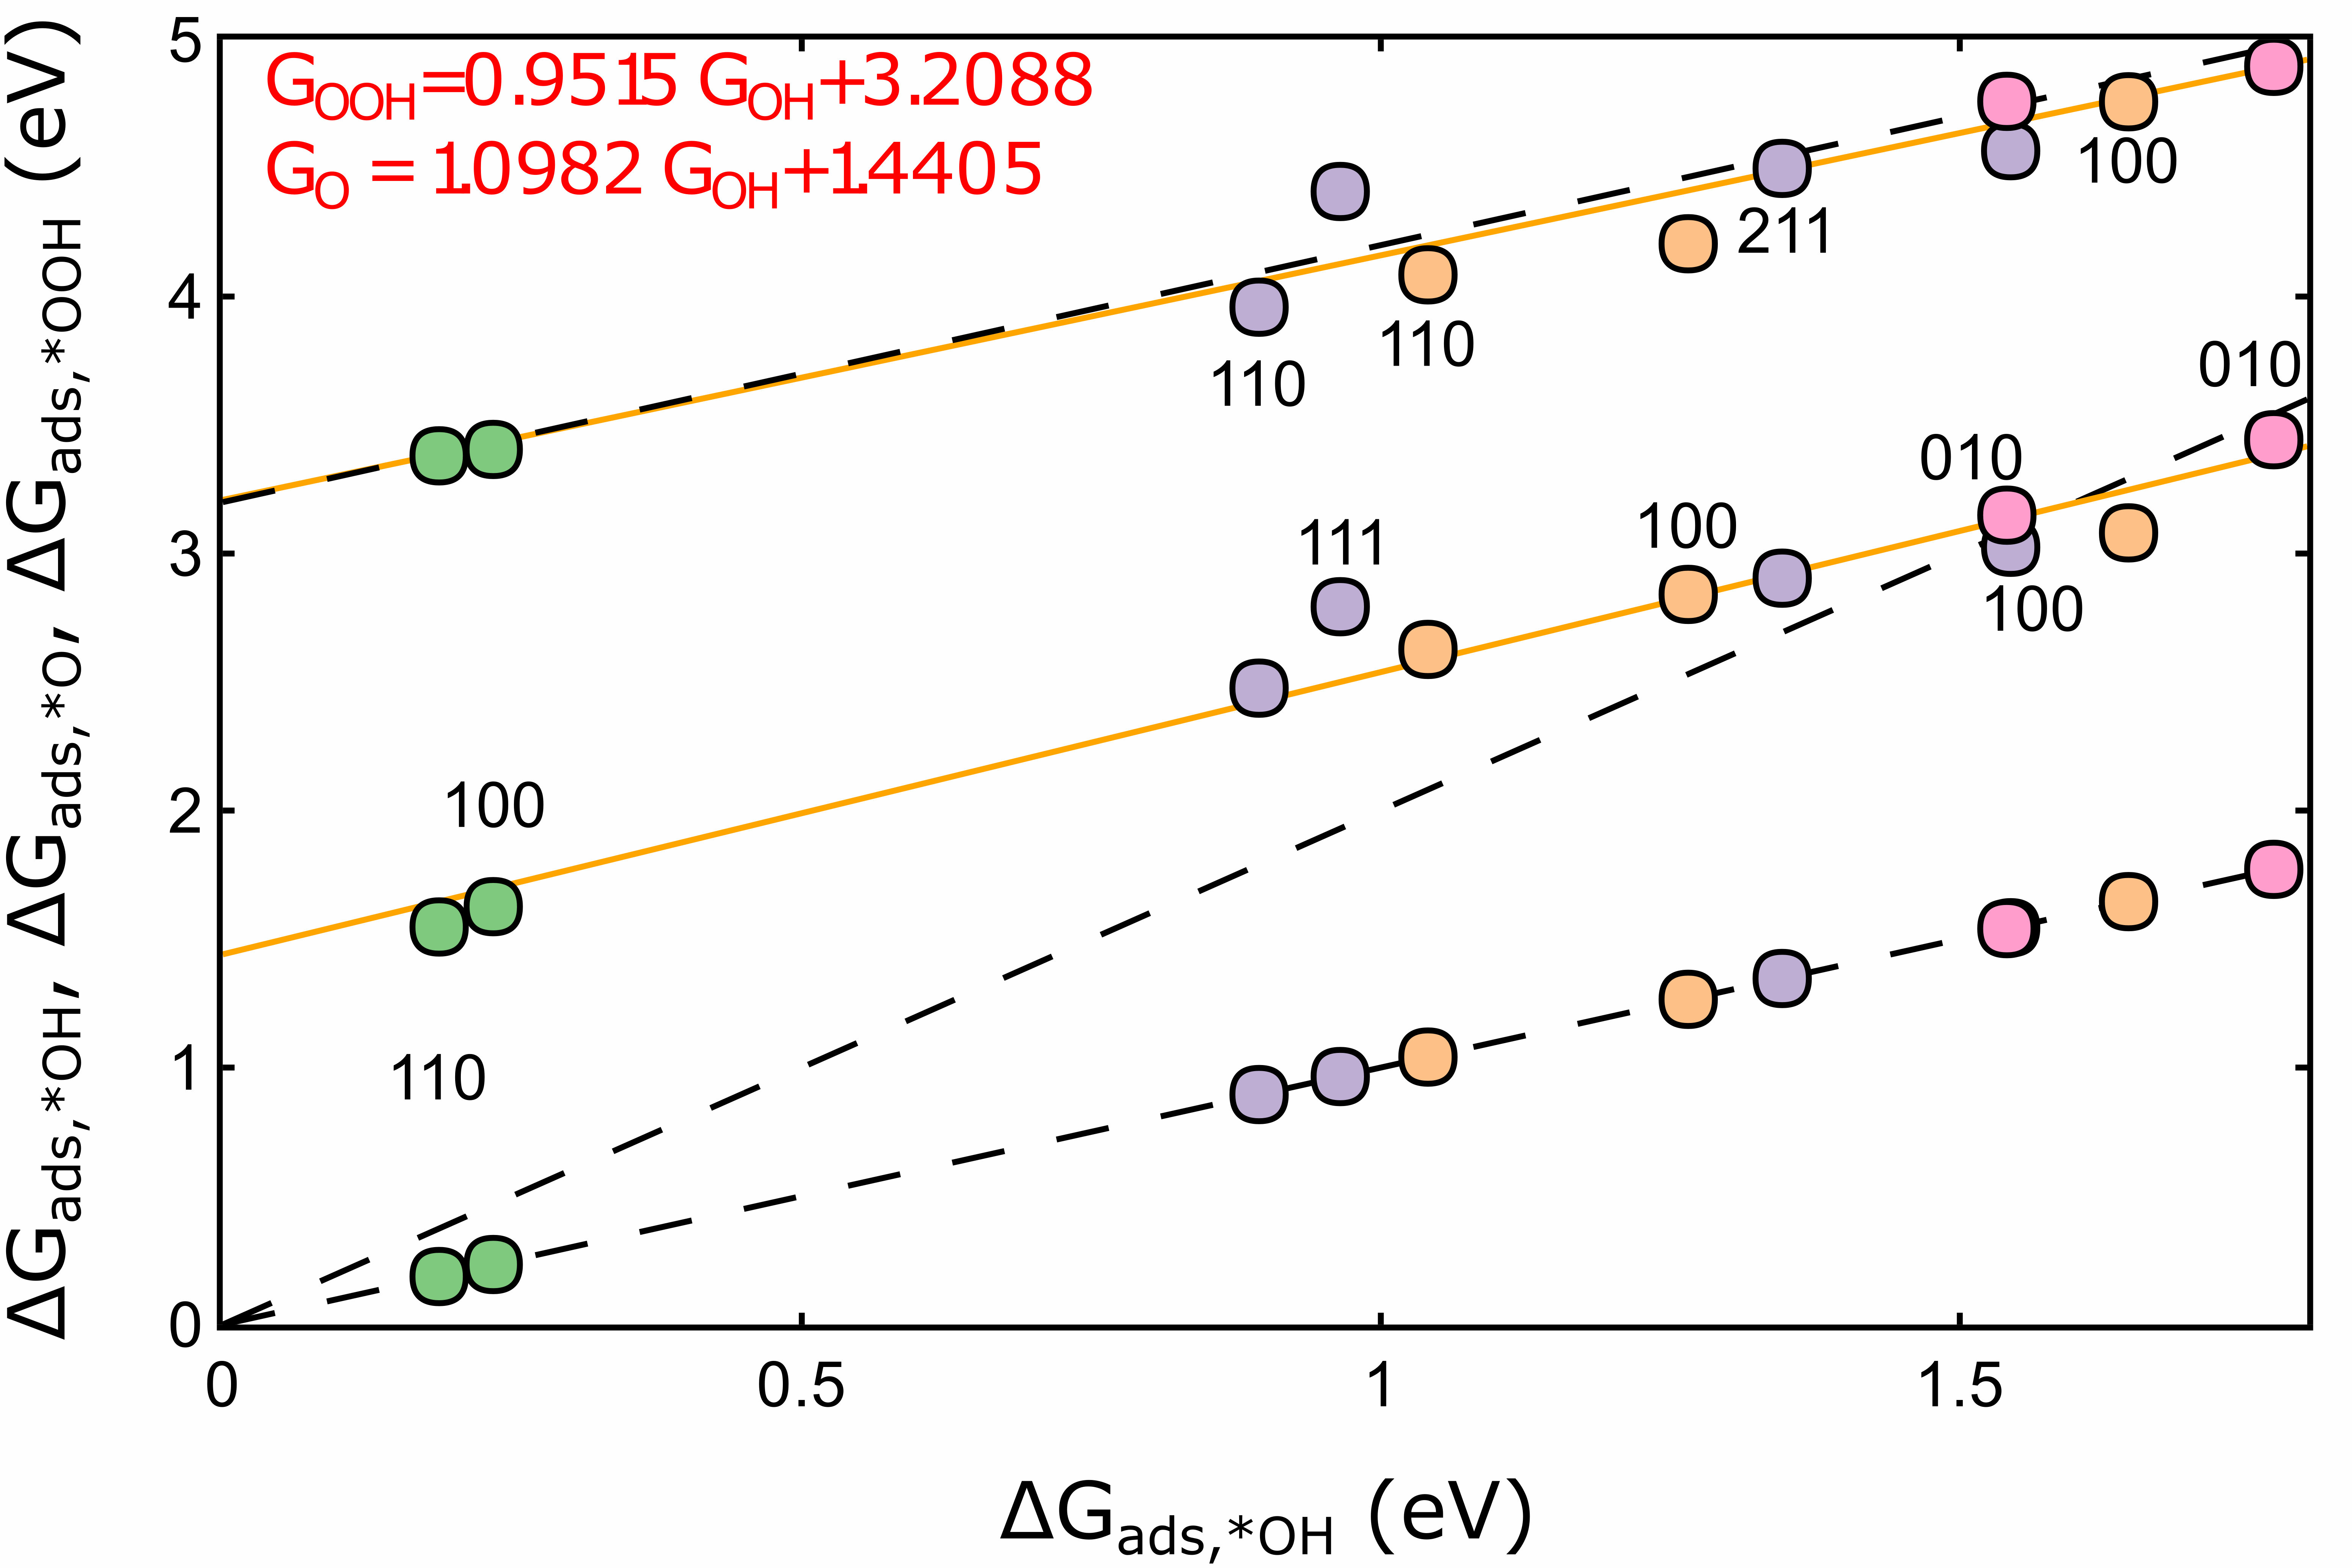
\includegraphics
{02_figures/oer_activity_stability/00_master__oer_scaling__main_v0__outplot2.png}
% {02_figures/oer_activity_stability/pl_scaling_relations_tmp.pdf}
}
\caption{\label{fig:scaling_relations}
% Adsorption free energy scaling relations plot.
Relationship between the adsorption free energies of the three key OER intermediates (*OH, *O, *OOH), with \DGOH chosen as the dependent variable.
Best fit lines are provided for \DGOOH vs. \DGOH and \DGO vs. \DGOH.
Additionally, ``universal scaling relations'' for \DGOOH vs. \DGOH and \DGO vs. \DGOH are shown (black dotted lines) to emphasize our deviation from the traditionally reported scaling fits.
The trivial \DGOH vs. \DGOH relationship is included for completeness.
% TODO Do I have to redefine the color convention every caption?
}
\end{figure}
% __|

% __|
